\section{ آشنایی با ابزارها و مجموعه داده}
این قسمت به معرفی ابزارهای استفاده شده در این پژوهش می‌پردازد. آشنایی با این ابزارها به درک هرچه بهتر  نحوه‌ی استخراج معیارها  و روند آزمایش کمک می‌کند.

\subsection{مجموعه داده \lr{defect4j}}
 مجموعه‌‌داده‌ی انتخابی به منظور انجام مورد مطالعاتی لازم است که دارای ویژگی‌های زیر باشد:
 \begin{itemize}
 	\item
 	اطلاعات خطاهای پروژه وجود داشته باشد و این اطلاعات نشان دهد که خطا متعلق به کدام فایل در کدام ثبت است. 
 	\item
 	پروژه‌ها متن-باز باشد تا بتوان با استفاده از کد منبع آنها معیارها را استخراج نمود.
 	\item
 	برای پروژه‌ها موارد آزمون مناسب وجود داشته باشد تا بتوان معیارهای جهش را استخراج کرد.
 \end{itemize}
 در میان مجموعه‌داده‌های موجود مجموعه‌داده‌ی \lr{defects4j} تنها موردی است که تمام ویژگی‌ها را دارد.\\
 
این مجموعه شامل  شش پروژه می‌باشد که پنج مورد از آن‌ها مربوط به شرکت \نام{آپاچی}{Apache} است و دیگری نرم‌افزار jfreechart است که به شرکت خاصی تعلق ندارد. این پروژه‌ها  \واژه{متن-باز} هستند و با استفاده از نرم‌افزارهای کنترل نسخه‌ی گیت و svn می‌توان به کدهای آن‌ها در طول فرآیند توسعه‌ی آنها دسترسی پیدا کرد.
مجموعه‌داده‌ی \چر{defect4j} به صورت یک \واژه{چهارچوب} ارائه شده است که کارهایی بیش از نگهداری اطلاعات درباره‌ی پروژه‌ها انجام می‌دهد. مهم‌ترین  کارهایی که می‌توان به وسیله‌ی این ابزار انجام داده عبارت است در جدول زیر آمده است. 


\begin{table}[H] 
	\renewcommand*{\arraystretch}{1.3}	
	\centering \caption{عملیات‌های موجود در \چر{defects4j}  }
	\label{tab:defects4j-ops}
	\newcolumntype{C}{>{\centering\arraybackslash} m } 
	\begin{tabular}{ |c|c|}
		
		\hline
		\hline
		نام عملیات  & توضیح
		\\
		\hline
		\hline
		\lr{info } &   نمایش پیکربندی یک پروژه‌ی خاص یا خلاصه‌ی یک خطای خاص
		\\
		\hline
		\lr{checkout} &   وارسی یک نسخه‌ی حاوی خطا یا تعمیر شده از پروژه
		\\
		\hline
		\lr{compile} &   کامپایل کدهای و آزمون‌های نوشته شده توسط توسعه‌دهندگان
		\\
		\hline
		\lr{test} &   اجرای یک آزمون یا مجموعه‌ی آزمون در یک نسخه‌ی حاوی خطا یا تعمیر شده از پروژه
		\\
		\hline
		\lr{mutation} &   اجرای تحلیل جهش در یک نسخه‌ی حاوی خطا یا تعمیر شده از پروژه
		\\
		\hline
		
	\end{tabular}
\end{table}

این ابزار در اجرای عملیات‌های بالا دارای محدودیت است و تنها آن‌ها را بر روی ثبت‌های از پیش تعیین شده انجام می‌دهد. ثبت‌های از پیش تعیین شده شامل ثبت‌های حاوی خطا و تعمیر آن خطا می‌باشد. در جدول زیر اطلاعات مربوط به تعداد خطاهای هر پروژه آمده است. 

\begin{table}[H] 
	\renewcommand*{\arraystretch}{1.3}	
	\centering \caption{پروژه‌های موجود در \چر{defects4j}  }
	\label{tab:defects4j-bugs}
	\newcolumntype{C}{>{\centering\arraybackslash} m } 
	\begin{tabular}{ |c|c|c|}
		
		\hline
		\hline
	نام مختصر &	نام کامل  & تعداد خطا
		\\
		\hline
		\hline
		\lr{Chart } & JFreeChart &	26
		\\
		\hline
		\lr{Closure} & \lr{Closure compiler}	& 133
		\\
		\hline
		\lr{Lang} &   \lr{Apache commons-lang} &	65
		\\
		\hline
		\lr{Math} &  \lr{Apache commons-math} &	106
		\\
		\hline
		\lr{Mockito} &   Mockito &	38
		\\
		\hline
		Time & Joda-Time &	27
		\\
		\hline
		
	\end{tabular}
\end{table}


به منظور نصب و راه اندازی این ابزار ابتدا از صفحه ی github آن پروژه بر روی  PC ، کلون می شود. سپس یک script باید اجرا کرد تا سایر تعلقات پروژه دانلود شود. این تعلقات شامل مخزن نرم افزاری مربوط به این این شش پروژه است که کدهای پروژه ها در آن قرار دارد. نکته ی قابل توجه در این پروژه این است بجز  دستور info سایر دستورات عملیاتهای مربوط را بر روی کامپیوتر کاربر انجام می‌دهند و خروجی را نمایش می‌دهند نه اینکه از یک پایگاه داده اطلاعات صرفاً بارخوانی شوند. 
در نیازمندی های این ابزار اشاره شده که باید از جاوا نسخه ی ۷ استفاده شود. اما مسأله ای که به آن اشاره نشده توزیع کننده ی جاوا است. جاوا دو توزیع کننده ی عمده دارد. یکی OpenJDK و دیگر Oracle. در ابتدا از نسخه ی openJDK استفاده شد زیرا نصب آن در linux ساده‌تر است و همچنین oracle به ایرانیان اجازه ی دانلود نمی دهد. اما با openJDK ابزار defects4j و ابزارهایی که به آن وابسته است به خوبی کار نمی کنند. به عنوان مثال برخی مجموعه تست ها که باید بدون خطا اجرا شوند به دلیل نبود dependency های لازم با شکست مواجه می شوند. این مسأله موجب سردرگمی و صرف مدت زمانی تا حل آن شد. 
راه ارتباط با این ابزار command line‌ می‌باشد و نمونه‌ ای از دستورات قابل استفاده در این ابزار  در شکل  \ref{fig:d4j-info-command} است که این دستور اطلاعات مربوط به پروژه ی Lang خطای شماره ی یک را خواهد داد. 
\begin{latin}
	\flushleft
defects4j info -p Lang -b 1
\end{latin}

\begin{figure}[H]
	\centering
	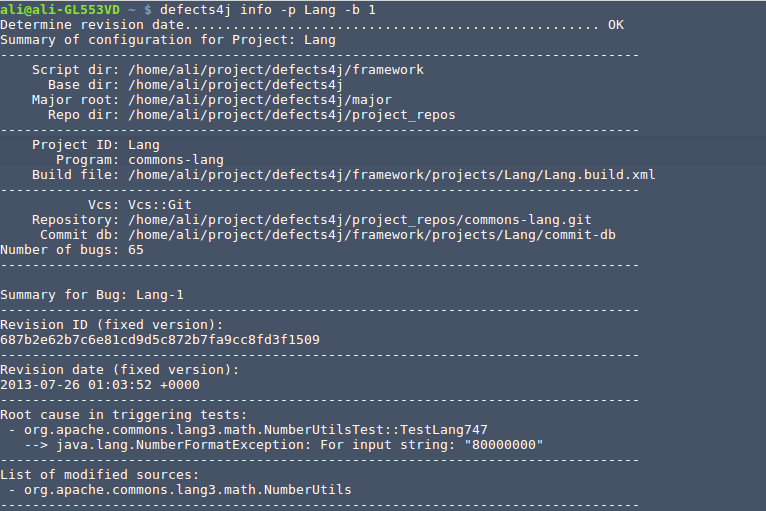
\includegraphics[width=.8\textwidth]{img/case_study/d4j-info-commadn.png}
	\caption{اجرای دستور info در \lr{defects4j}}
	\label{fig:d4j-info-command}
\end{figure}

\subsection{ابزار Major}

این ابزار جهت تولید جهش یافته و تحلیل جهش استفاده می شود. در ابتدا تصمیم بر این بود از ابزار دیگری به نام PIT استفاده شود ولی ابزارdefect4j از major استفاده می‌کند بنابرین به دلیل سازگاری با D4j و نیز قابلیت‌های منحصر به فرد این ابزار تصمیم به استفاده از Major  گرفته شد. چند مورد از ویژگی‌ها عبارتند از :
\begin{itemize}

\item
 راحتی استفاده: قابلیت تعامل از روشهای مختلف مانندcommand lineِ، بکارگیری به وسیله ی ابزار build ant و دستورات کم نسبت به PIT
\item
 مجموعه عملگرهای کاملتر
\item
 راحتی در پیکر بندی : امکان انجام تحلیل تنها برای یک کلاس یا تابع، تنظیمات راحت و کامل جهت مشخص کردن مجموعه عملگرها
\end{itemize}
لازم به ذکر است که این ابزار از compiler‌ مخصوص به خود جهت کامپایل برنامه و ساخت جهش یافته استفاده می‌کند که گسترش یافته ی یک کامپایلر جاوا است. 
البته در انتها مشخص شد که این برنامه کاستی هایی هم دارد از جمله کامل نبود مستندات برای بکارگیری پیشرفته و خطاهایی که در قسمت مربوطه به آن‌ها اشاره خواهد شد. 
استفاده از این ابزار را می‌توان در سه مرحله خلاصه کرد :
\begin{enumerate}
\item

پیکربندی تولید جهش یافته به وسیله MML script: این ابزار برای مشخص نمودن اینکه از چه عملگرهای استفاده شود و آن‌ها در چه محل هایی از برنامه به کار گرفته شوند یک زبان ساده ابداع کرده است به نام MML که یک کامپایلر نیز دارد. ابتدا کد mml نوشته می‌شود سپس با mmlc کامپایل می‌شود و نتیجه به عنوان یکی از پارامترها به در هنگام فراخوانی ابزار ارسال می شود. نمونه‌ای از این کد در شکل \ref{fig:major-mml} آمده است. 

\begin{figure}[H]
	\centering
	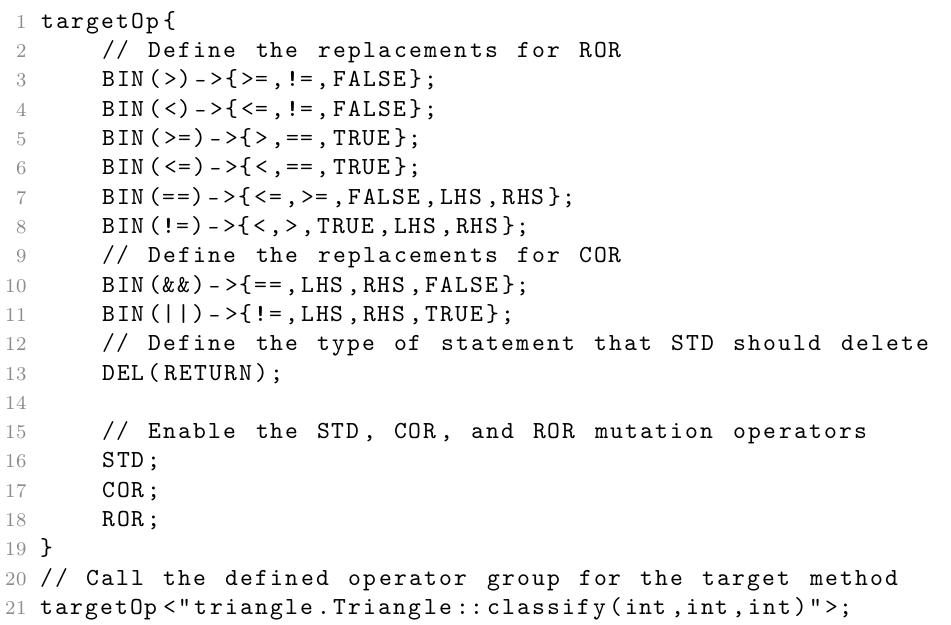
\includegraphics[width=.8\textwidth]{img/case_study/major-mml.png}
	\caption{نمونه کد MML در Major}
	\label{fig:major-mml}
\end{figure}
\item 	
تولید جهش یافته ها: برای این منظور می‌توان از command line یا فایل build.xml مربوط به پروژه استفاده کرد که روش دوم مورد استفاده قرار گرفت. برای این منظور لازم است که یک قطعه کد به شکل زیر به فایل build.xml اضافه شود. و سپس برنامه کامپایل شود. حاصل به شکل زیر خواهد بود که نشان می‌دهد ۸۶ جهش یافته تولید شده است. همچینین ابزار یک فایل به نام mutation.log تولید می‌کند که نشان می‌دهد چه جهش یافته هایی در کجا تولید شده اند. 

\begin{figure}[H]
	\centering
	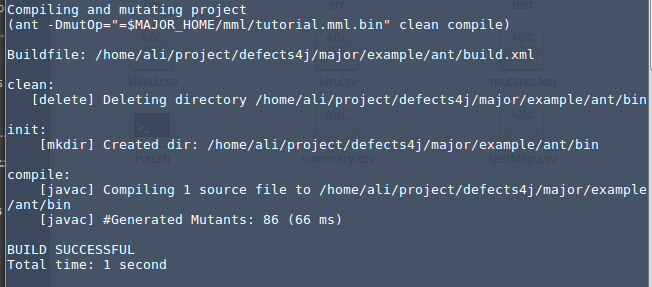
\includegraphics[width=.8\textwidth]{img/case_study/major-mutant.png}
	\caption{نمونه کد MML در Major}
	\label{fig:major-mutant}
\end{figure}

\begin{figure}[H]
	\centering
	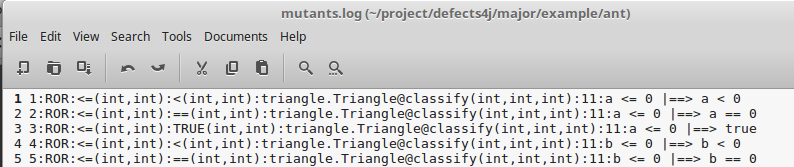
\includegraphics[width=.8\textwidth]{img/case_study/major-log.png}
	\caption{نمونه کد MML در Major}
	\label{fig:major-log}
\end{figure}

\item
 اجرای تحلیل جهش : در این قسمت نیز قطعه کدی به فایل build.xml اضافه می‌شود و سپس فایل اجرا می شود. در اجرا ابتدا فایل‌های تست کامپایل می‌شود و سپس هر مجموعه تست بر روی جهش یافته هایی که تا کنون کشته نشده‌اند اجرا می شود. در پایان نتایج را در خروجی چاپ می کند. همچنین نتایج را در فایلهای با پسوند csv قرار می دهد. نمونه‌ای از اجرای تحلیل جهش و فایلهای خروجی در زیر آمده است:
 
 \begin{figure}[H]
 	\centering
 	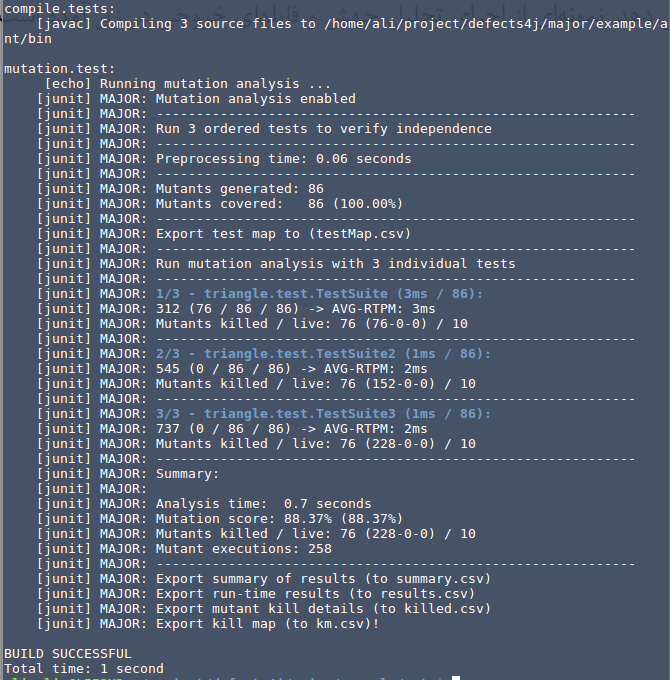
\includegraphics[width=.8\textwidth]{img/case_study/major-analysis.png}
 	\caption{نمونه کد MML در Major}
 	\label{fig:major-analysis}
 \end{figure}
 
 \begin{figure}[H]
 	\centering
 	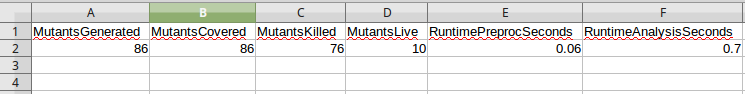
\includegraphics[width=.8\textwidth]{img/case_study/major-results.png}
 	\caption{نمونه کد MML در Major}
 	\label{fig:major-results}
 \end{figure}

\end{enumerate}


\subsection{کتابخانه‌ی Jgit}
این کتابخانه جهت کار با مخازن نرم افزاری از نوع git به کار گرفته می‌شود و به زبان جاوا است. تمام عملیات های مهم و اساسی که در نرم‌افزار اصلی git وجود دارد در این کتابخانه نیز قابل انجام است. مشکلی که کار با این کتابخانه دارد نبود منابع آموزشی به اندازه ی کافی است. چراکه کاربران زیادی ندارد و آموزش‌های ابتدایی معمولاً نیازهایشان را بر طرف می کند. 
\subsection{چهارچوب Hibernate }
به وسیله ی این چارچوب می‌توان  اشیاء موجود در برنامه ی جاوا را به داده‌های موجود در پایگاه داده تبدیل کرد. اصطلاحاً به این ابزار ها ORM (object relational mapping)  می گویند. در ابتدا تصمیم بر این بود که داده‌های بدست آمده در فایل متنی ذخیره شوند و در هنگام نیاز آن‌ها خوانده شوند یا همه ی اشیاء با هر بار اجرا ساخته شوند نکات زیر سبب شد که هزینه ی اول کار با پایگاه داده و مزایای بلند مدت آن به سادگی استفاده از فایل متنی ترجیح داده شود:
۱- هر بار ساخت اشیاء با اجرای برنامه بسیار زمانبر است و اتلاف وقت زیادی دارد
۲- لازم است برای اطمینان از درستی برنامه، داده‌ها در قالب جداولی به صورت چشمی کنترل شوند
۳- فراخوانی و جستجو در پایگاه داده سریع است و کارایی بالا می‌رود
۴- نگهداری از برنامه در دراز مدت راحت‌تر خواهد بود و خوانایی کدها بیشتر خواهد بود چرا که کار با پایگاه داده دارای اصول مشخصی است و سایرین از آن اطلاع دارند اما فایل متنی اینگونه نیست
